\documentclass[11pt,letterpaper,titlepage]{article}
\usepackage[utf8]{inputenc}

% AMSmath and more
\usepackage{mathtools}

% Blackbox
\usepackage{amssymb}

% Nicer SI Units
\usepackage{siunitx}
\sisetup{number-unit-product = \:, inter-unit-product = \:, parse-numbers = false, detect-weight=true, detect-family=true}

% Clickable links
\usepackage{hyperref}

% Text spacing
\usepackage{microtype}

% % Space between paragraphs instead of indentation
% \usepackage{parskip}

% % Required to make parskip compatible with amsthm
% \makeatletter
% \def\thm@space@setup{%
%   \thm@preskip=\parskip \thm@postskip=0pt
% }
% \makeatother

% Figures go HERE
\usepackage{float}

% Sub-figures
\usepackage{subcaption}

% Nicer tables
\usepackage{booktabs}

% Enables \mathscr for script letter in math mode
\usepackage{mathrsfs}

% TikZ for drawing diagrams
\usepackage[dvipsnames]{xcolor}
\usepackage{pgf,tikz}
\usetikzlibrary{arrows}
\usetikzlibrary{decorations.markings}
\usetikzlibrary{matrix}

% Nicer pseudo code
\usepackage{algorithm}
\usepackage[noend]{algpseudocode}

% Syntax highlighting
\usepackage{minted}
\usemintedstyle{pastie}

% Enables the \ce command for chemical formulas and equations
\usepackage[version=4]{mhchem}

% Add bibliography to TOC
\usepackage[nottoc,numbib]{tocbibind}

% Change how numbering should be done 
% (default is single positive integers, choosing 
% 'section' will include the section number, choosing
% 'subsection' will include subsection number etc.) 
\numberwithin{equation}{section}
\numberwithin{figure}{section}
\numberwithin{table}{section}
\numberwithin{algorithm}{section}

% Proof (and custom) environments
\usepackage{amsthm}

\theoremstyle{definition}
\newtheorem{theorem}{Theorem}[section] % theorem numbers will include section number
\newtheorem{definition}[theorem]{Definition} % definitions will share numbering with theorems
\newtheorem{fact}[theorem]{Fact} % etc.
\newtheorem{proposition}[theorem]{Proposition}
\newtheorem{example}[theorem]{Example}
\newtheorem{remark}[theorem]{Remark}
\newtheorem{claim}[theorem]{Claim}
\newtheorem{joke}[theorem]{Joke}

% Makes it possible to combine \textbf with other environments (in particular math environments)
\usepackage{bm}
\makeatletter
\g@addto@macro\bfseries{\boldmath}
\makeatother

% Own math operators
\DeclareMathOperator{\col}{col}
\DeclareMathOperator{\spn}{span}

% Macros
\newcommand{\N}{\mathbb{N}}
\newcommand{\Z}{\mathbb{Z}}
\newcommand{\Q}{\mathbb{Q}}
\newcommand{\R}{\mathbb{R}}
\newcommand{\C}{\mathbb{C}}
\newcommand{\Qu}{\mathbb{H}}
\newcommand{\Oc}{\mathbb{O}}
\newcommand{\dx}{\,\mathrm{d}x}

\newcommand{\bb}[1]{\mathbb{#1}}
\newcommand{\ff}[2]{\mathbb{F}_{#1^{#2}}}
\newcommand{\gl}[2]{\mathrm{GL}_{#1}(\mathbb{#2})}

% -----------------------------% 
\title{\vspace{-2in} \huge Intermediate {\LaTeX} Topics in Action}
\author{\Large Zack Garza and Oskar Henriksson}
\date{\Large \today}


\usemintedstyle{pastie}
\begin{document}

\maketitle
\thispagestyle{empty} % suppress page-numbering
\tableofcontents
\newpage
\setcounter{page}{1} % start counting from the first page

% -----------------------------% 
\section{Math hackery}
In this section, we show a few examples of tricks that aren't necessary to get started with \LaTeX, but still are very useful in mathematical writing. 

Throughout this section (and some of the sections to come) we use the \verb$amsthm$ package to keep track of theorems, definitions, and proofs. It might also be a good idea to use \verb$\newcommand$ and \verb$\DeclareMathOperator$ to create macros for certain symbols and operators that come up a lot.

\subsection{Alignment and spacing}
\label{su:alignment}
Our first examples will feature various ways to adjust spacing various ways to adjust spacing (using commands like \verb$\:$, \verb$\,$ and \verb$\!$) and align objects horizontally and vertically (using environments such as {\verb$pmatrix$}, {\verb$align*$} and {\verb$cases$}, as well as the commands {\verb$&$} and \verb$\\$). 

The commands \verb$\mathrm$, \verb$\text$ and \verb$\operatorname$ also come up, as a way of including text in math mode.

\begin{theorem}
    The quadratic equation $ax^2+bx+c=0$, where and $b,c\in\mathbb{R}$ and $a\in\mathbb{R}\setminus \{0\}$ has the solutions
    \[
    x_1 = \frac{-b+\sqrt{b^2-4ac}}{2a}
    \:\:\:\text{and}\:\:\:
    x_2 = \frac{-b-\sqrt{b^2-4ac}}{2a}\,.
    \]
\end{theorem}

\begin{proof}
Left as an exercise for the reader.
\end{proof}

\begin{definition} The \emph{column space} of a matrix $A = (a_{ij})\in\R^{m\times n}$ is given by
\[
\col(A)=
\col\begin{pmatrix}
a_{11} & \cdots & a_{12}\\
\vdots & \ddots & \vdots\\
a_{m1} & \cdots & a_{mn}
\end{pmatrix}
=
\spn\left\{
    \begin{pmatrix}
        a_{11}\\\vdots\\a_{m1}
    \end{pmatrix}
    , \, \ldots \, ,
    \begin{pmatrix}
        a_{1n}\\\vdots\\a_{mn}
    \end{pmatrix} 
\right\}\,.
\]
\end{definition}

\begin{definition}
The \emph{sign function} is the function $\operatorname{sgn}\colon \R\to\R$ defined by

\[
\operatorname{sgn}(x):=
\begin{cases}
1   &\text{if $x>0$}\\
0   &\text{if $x=0$}\\
-1  &\text{if $x<0$\,.}
\end{cases}
\]

\end{definition}

\begin{theorem}
\label{thm:cubic}
Let $x,y\in \R$. Then $(x+y)^3=x^3+3x^2y+3xy^2+y^3$.
\end{theorem}

\begin{proof}[Proof (using formula for square of binomial)]
\begin{align*}
(x+y)^3 &=(x+y)(x+y)^2\\
        &=(x+y)(x^2+2xy+y^2)\\
        &=x^3+2x^2y+xy^2+xy^2+2xy^2+y^3\\
        &=x^3+3x^2y+3xy^2+y^3\,.\tag*{\qedhere}
\end{align*}
\end{proof}

\subsection{Text in math mode and other math hacks}
We will now turn our focus to text, and more ways in which text  be added in math environments. We will, again, use \verb$\text$ and \verb$\mathrm$ for this, but also introduce the \verb$\SI$ command for units, and the \verb$\ch$ command for chemical equations. Both of these come from special packages.

We will also play around with fancy letters (\verb$\mathcal$ and \verb$\mathscr$ are useful for this), adding stuff over/under objects in math mode (eg. using the \verb$\overbrace$ and \verb$\overset$ commands) or adding color (using \verb$\color$).

\begin{proposition}The set $\mathscr{C}^0[a,b]:=\{f\colon [a,b]\to \R: \text{$f$ is continuous}\}$ is a vector space under point-wise addition and scalar multiplication.
\end{proposition}

\begin{proposition}
$\mathscr{U}$, $\mathbb{C}$, $\mathcal{S}$, $\mathfrak{D}$, as well as $\mathcal{S}$, $\mathscr{U}$, $\mathfrak{M}$ and $\mathbb{S}$, are cool letters.
\end{proposition}

\begin{remark}
Let $a\in \R$ and let $m,n\in\mathbb{Z}^+$. Then  we have
\[a^m\cdot a^n=(\overbrace{a\cdots a}^{\text{$m$ factors}})\cdot (\overbrace{a\cdots a}^{\text{$n$ factors}})\overset{(*)}{=}\overbrace{a\cdots a\cdot a\cdots a}^{\text{$m+n$ factors}}=a^{m+n}\,,\]
where $(*)$ follows from the associative law.
\end{remark}

\begin{remark} A $u$-substitution can sometimes simplify an integral a lot:
\[
\int_0^2 x\sin(x^2+1) \,\mathrm{d}x
=\frac{1}{2}\int_0^2 {\color{MidnightBlue}2x}\sin({\color{BrickRed}x^2+1}) \,{\color{MidnightBlue}\mathrm{d}x}=
\frac{1}{2}\int_1^5\sin({\color{BrickRed}u}) \,{\color{MidnightBlue}\mathrm{d}u}\,.
\]
\end{remark}

\begin{joke}
If $\displaystyle\lim_{x\to 8^+}\frac{1}{x-8}=\infty$\,, then $\displaystyle\lim_{x\rightarrow5^+}\frac{1}{x-5}=\rotatebox{90}{5}$\,.
\end{joke}

\begin{fact}
One of the authors has mass $m = \SI{74}{\kilo\gram}$. Converted to pure energy, that corresponds to 
\[
E=mc^2
=(\SI{75}{\kilo\gram}) (\SI{2.99\cdot10^8}{\meter\per\second})^2
=
\SI{6.651\cdot10^{18}}{\joule}
\,.
\]
\end{fact}

\begin{fact}
If acetic acid is dissolved in \SI{2}{\deci\meter\cubed} water, and \SI{0.01}{\mol} of the acid dissociates according to
\[
\ce{CH3COOH + H2O <=> H3O+ + CH3CO2^-}\,,
\]
we obtain 
\[
\mathrm{
    \mathit{c}(H_3O^+)
    =
    \frac{\SI{0.01}{\mol}}{\SI{2}{\deci\meter\cubed}}
    =
    \SI{0.005}{\mole\per\deci\meter\cubed}
}\,.
\]
\end{fact}




% -----------------------------% 
\section{Tables}
    
\begin{fact}
    A day is \emph{much} longer on Mercury than here on Earth. For more facts like this, refer to the table below:
\end{fact}
    
\begin{table}[H]
    \centering
    \caption{Data for the terrestrial planets. \label{tbl:planets}} 
    \begin{tabular}{llll}
        \toprule
        \textbf{Planet}     &\textbf{Mass (\si{\kilo\gram})}    & \textbf{Density (\si{\kilo\gram\per\meter\cubed})} & \textbf{Length of Day (\si{\hour})}\\
        \midrule
        Mercury & $3.30\times 10^{23}$  & 5\,427 & 4\,222.6\\
        Venus     & $4.86\times 10^{24}$ & 5\,243 & 2\,802.0    \\
        Earth    & $5.97\times 10^{24}$ & 5\,514 & 24.0 \\
        Mars    & $6.42\times 10^{23}$ & 3\,933 & 24.7\\
        \bottomrule
    \end{tabular}
\end{table}

\begin{theorem}[De Morgan's Laws]
    For statements $p$ and $q$, it holds that \[\neg\,(p\wedge q)\iff (\neg\, p)\vee (\neg\, q)\:\:\:\text{and}\:\:\:\neg\,(p\vee q)\iff (\neg\, p)\wedge (\neg\, q)\,.\]
\end{theorem}

\begin{proof}[Proof (of the first equivalence)]
    Consider the following truth table:
\begin{center}
\begin{tabular}{ccccccc}
    \toprule
    \textbf{$p$} & \textbf{$q$} & \textbf{$p\wedge q$} & \textbf{$\neg\,(p\wedge q)$} & \textbf{$\neg\, p$} & \textbf{$\neg\, q$} & \textbf{$(\neg\,p)\vee (\neg\, q)$} \\
    \midrule
    T & T & T & F & F & F & F\\
    T & F & F & T & F & T & T\\
    F & T & F & T & T & F & T\\
    F & F & F & T & T & T & T\\
    \bottomrule
\end{tabular}
\end{center}
The desired result follows from the fact that $\neg\,(p\wedge q)$ and $(\neg\, p)\vee (\neg\, q)$ have the same truth value on every row of the truth table.
\end{proof}


% -----------------------------% 
\section{Labels and cross-referencing}

{\LaTeX} does not only keep track of the numbering of pages, sections, figures, equations, theorems, and references, it also makes it very easy to refer back to them whenever we want.

\subsection{Back-references to equations, sections, figures etc.}
Here we focus specifically on numbered objects and how we can refer back to them using the commands \verb$\label$ and \verb$\ref$.
 
\begin{theorem}
    \label{thm:binomial}
    Let $x,y\in\R$ and $n\in\Z^+$. Then
    \begin{equation}
        \label{eq:binomial}
        (x+y)^n=\sum_{k=0}^n\binom{n}{k}x^ky^{n-k}\,.
    \end{equation}
\end{theorem}    

\begin{proof}
    The idea we used in the proof of Theorem~\ref{thm:cubic} (in Section~\ref{su:alignment}) can be adapted to prove this theorem by induction over $n$.  
\end{proof}

\begin{remark}
Plugging in $x=y=1$ in Equation~\ref{eq:binomial} shows that we, for every $n\in\Z^+$, have 
\[\binom{n}{0}+\binom{n}{1}+\cdots+\binom{n}{n}=2^n\,.\]
\end{remark}

\begin{fact}
    The torus is a very interesting topological object; Figure~\ref{fig:torus} shows the magnificent torus in its natural habitat.
\end{fact}

\begin{figure}[H]
    \centering
    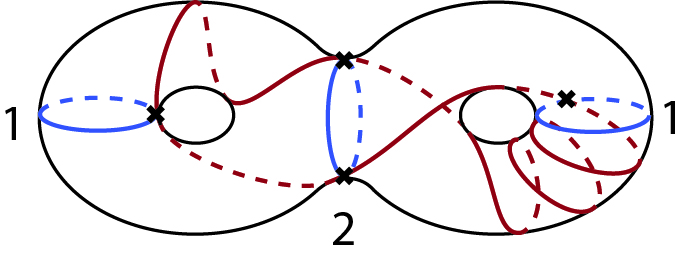
\includegraphics[width=0.3\linewidth]{top1}
    \caption{A torus.}
    \label{fig:torus}
\end{figure}
    
\subsection{Back-referencing page numbers}
{\LaTeX} also makes it possible to refer to the page number at which some numbered object appeared via the command \verb$\pageref$. We can, for example, talk about what we learned in Section~\ref{su:alignment} on page~\pageref{su:alignment}, Theorem~\ref{thm:binomial} on page~\pageref{thm:binomial}, or Figure~\ref{fig:torus} on page~\pageref{fig:torus}.

\begin{fact}
    Mars is less dense than Venus (cf. Table~\ref{tbl:planets} on page~\pageref{tbl:planets}).
\end{fact}
  
\subsection{Footnotes}

Another handy referencing feature is the ability to include footnotes in your documents. The footnote itself is written right in the source code where you want it to appear, and the compiler takes care of any placement and numbering issues. For example:

\begin{theorem}
Given a topological space, $M$, a \textit{chart}\footnote{\label{myFootnoteName}Also referred to as a \textit{local coordinate map} in some texts.} is a pair $(U, \phi)$, where $U \subseteq M$ is open and $\phi: U \rightarrow \Omega$ is a homeomorphism
onto an open subset, $\Omega := \phi(U) \subseteq R^n$ for some $n \geq 1$.
\end{theorem}

%You can also give it a label name (much like for equations), and refer to it later: ``See footnote~\ref{myFootnoteName}.''

\subsection{Bibliography}
At the end of this document is a bibliography (created using the \verb$thebibliography$ environment) containing an actual list of useful references. For example, by using the \verb$\cite$ command, you can refer to \cite{tables} to learn more about tables. 

You can also refer to specific chapters and pages:

\begin{quote}
... extra spaces between words have no particular meaning for {\TeX} ... for the virtuoso typist, some of these features might seem unnecessary, or even down-right perverse. \cite[chapter 1, p.~7]{joyoftex}
\end{quote}
  
% -----------------------------% 
\section{Source Code}

There are several ways to include a program's source code in your documents; here we cover a few common use cases.

 \subsection{Plain pseudo-code}
 
 For topics such as Data Structures or Algorithms, it's often desirable to communicate the logic of a function or procedure in a language-agnostic way. Fortunately, there are several packages that facilitate writing pseudo-code. 
 
 Here we use the \verb$algorithmicx$ package to describe an algorithm for depth-first search in a graph $G$ with starting at a vertex $v_0$. 
 
    % algorithmi package
    \begin{algorithm}[H]
    \caption{Dijkstra's Algorithm}\label{Dijkstra}
    \begin{algorithmic}[1]
    \Procedure{Dijkstra($G$, $v_0$)}{}
    \For{each vertex $v \in V(G)$}
        \State $\text{dist}[v] \gets \infty$
        \State $\textit{prev}[v] \gets 0$
        \State $\text{dist[source]} \gets 0$
        \State $Q \gets \{v \mid v\in V(G)\}$
        \While{$Q \neq \varnothing$} 
            \State{$u \gets$ node in Q with smallest distance}
            \State{remove $u$ from $Q$}
            \For{each neighbor $v$ of $u$}
                \State{alt $\gets$ dist[$u$] + dist$(u, v)$}
                \If{alt $<$ dist[$v$]}
                    \State{dist[$v$] $\gets$ alt}
                    \State{\textit{prev}[$v$] $\gets u$}
                \EndIf
            \EndFor
        \EndWhile
    \EndFor
    \State{return \textit{prev}}
    \EndProcedure
    \end{algorithmic}
    \end{algorithm}
    
    %A very handy feature of this package is that each pseudo-code operator (such as the \textbf{while} loop) is created with a command, which gives you a weak form of syntax checking using the \TeX compiler.

 \subsection{Syntax highlighting}
 
 At other times, you may want to write out a full implementation in a specific language. In these cases, it is quite useful to have language-specific syntax highlighted to make code more legible.
 
 \begin{example}
 We can always type or copy-paste code directly into the document, and have \verb$minted$ take care of styling it:
 
    \begin{minted}
    [
    frame=lines,
    framesep=2mm,
    baselinestretch=1.2,
    fontsize=\footnotesize,
    linenos
    ]
    {python}
        import numpy as np
         
        def incmatrix(genl1,genl2):
            m = len(genl1)
            n = len(genl2)
            M = None #to become the incidence matrix
            VT = np.zeros((n*m,1), int)  #dummy variable
         
            #compute the bitwise xor matrix
            M1 = bitxormatrix(genl1)
            M2 = np.triu(bitxormatrix(genl2),1) 
         
            for i in range(m-1):
                for j in range(i+1, m):
                    [r,c] = np.where(M2 == M1[i,j])
                    for k in range(len(r)):
                        VT[(i)*n + r[k]] = 1;
                        VT[(i)*n + c[k]] = 1;
                        VT[(j)*n + r[k]] = 1;
                        VT[(j)*n + c[k]] = 1;
         
                        if M is None:
                            M = np.copy(VT)
                        else:
                            M = np.concatenate((M, VT), 1)
         
                        VT = np.zeros((n*m,1), int)
         
            return M
    \end{minted}
    \end{example}
    
    Note that you have to tell \verb$minted$ what language the file is written in (it has built-in support for quite a large number of languages out of the box).
   
   
 \subsection{Import file contents directly}
 
 However, no one likes to repeat themselves! Typing code into a document can be error-prone, and must be manually changed if the code is updated. If you already have a program's source in a file, its entire text content of the file can be imported and styled automatically. 
 
 \begin{example}
 Here we import an Octave script directly from a file:
 
 \inputminted{Octave}{source.code}
 \end{example}
 
 
 
% -----------------------------% 
\section{Diagrams using TikZ}
   \url{https://www.sharelatex.com/learn/TikZ\_package}


\begin{proposition} 
    This is the solution set of $x^2-9>0$ : 
    
    \begin{center}
    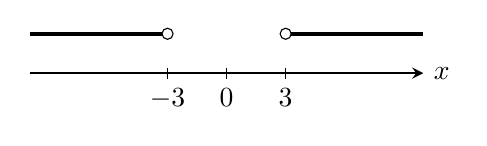
\begin{tikzpicture}[>=stealth,x=0.25cm]
    
    % x axis
    \draw[->,color=black, thick] (-10,0) -- (10,0) node[right] {$x$};
    \foreach \x in {-3,0,3}
    \draw[shift={(\x,0)},color=black] (0pt,2pt) -- (0pt,-2pt) node[below] {$\x$};
    
    \draw[line width=1.5] (-3,0.5) -- (-10,0.5); 
    \fill[color=white] (-3,0.5) circle (2pt);
    \draw[color=black] (-3,0.5) circle (2pt);
    
    \draw[line width=1.5] (3,0.5) -- (10,0.5); 
    \fill[color=white] (3,0.5) circle (2pt);
    \draw[color=black] (3,0.5) circle (2pt);
    \end{tikzpicture}
    \end{center}
\end{proposition}

\begin{fact}
    The following category theoretical diagram is an important part of the definition of the tensor product:
    \begin{center}
    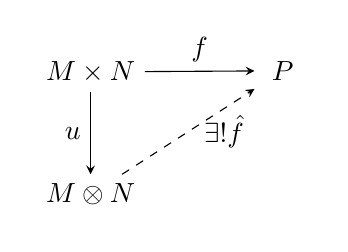
\begin{tikzpicture}
      \matrix (m) [matrix of math nodes,row sep=3em,column sep=4em,minimum width=2em]
      {
         M\times N & P \\
         M\otimes N &  \\};
      \path[-stealth]
        (m-1-1) edge node [left] {$u$} (m-2-1)
        (m-1-1) edge node [above] {$f$} (m-1-2)
        (m-2-1) edge [dashed] node [right] {$\:\exists ! \hat{f}$} (m-1-2);
    \end{tikzpicture}
    \end{center}
\end{fact}

\begin{fact}
    Linear optimization is essentially just a matter of systematically looking for minima or maxima among the vertices of a convex polygon in $\R^n$. In this 2-dimensional case, the function $f$ (a single, blue level curve is included in the plot) is maximized at the point $A$:

    \begin{figure}[H]
        \centering
        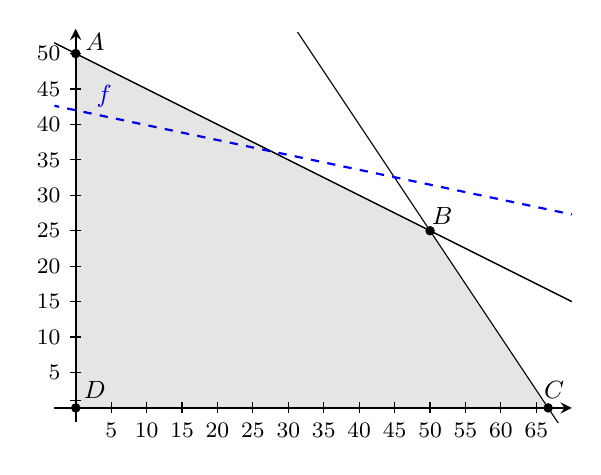
\begin{tikzpicture}[>=stealth,x=0.09cm,y=0.09cm]

            % x axis
            \draw[->,color=black, thick] (-3.,0.) -- (70,0.);
            \foreach \x in {5,10,15,20,25,30,35,40,45,50,55,60,65}
            \draw[shift={(\x,0)},color=black] (0pt,2pt) -- (0pt,-2pt) node[below] {\footnotesize $\x$};

            % y axis
            \draw[->,color=black, thick] (0.,-2) -- (0.,53.5);
            \foreach \y in {,5,10,15,20,25,30,35,40,45,50}
            \draw[shift={(0,\y)},color=black] (2pt,0pt) -- (-2pt,0pt) node[left] {\footnotesize $\y$};

            % Define the drawing area
            \clip(-3,-2) rectangle (70,53);

            % Plot the lines
            \draw [domain=-3.5:70] plot(\x,{(-200.--3.*\x)/-2.});
            \draw [domain=-3.5:70] plot(\x,{(-100.--1.*\x)/-2.});

            \draw [domain=-3.5:70] plot(\x,{(-100.--1.*\x)/-2.});

            \draw [thick, dashed,blue,domain=-3.5:70] plot(\x,{((42*(200-\x))/200});
            \draw[color=blue] (4,44) node {\small $f$};

            \draw [fill=black] (50.,25.) circle (1.5pt);
            \draw[color=black] (51.7,27.1) node {\small $B$};

            \draw [fill=black] (66.66666666666667,0.) circle (1.5pt);
            \draw[color=black] (67.5,2.5) node {\small $C$};

            \draw [fill=black] (0.,0.) circle (1.5pt);
            \draw[color=black] (2.7,2.5) node {\small $D$};
            
            \draw [fill=black] (0.,50.) circle (1.5pt);
            \draw[color=black] (2.7,51.7) node {\small $A$};

            % Plot the grey area
            \fill[color=black,fill=black,fill opacity=0.1] (0.,50.) -- (50.,25.) -- (66.66666666666667,0.) -- (0.,0.) -- cycle;

        \end{tikzpicture}       
        \caption{Constrained linear optimization in action.}
    \end{figure}
\end{fact}


% -----------------------------% 
\section{Customization}
    \subsection{Creating your own macros}
    If you find yourself stuck using long, cumbersome, or unintuitively named commands repeatedly, it is often useful to assign your custom shortcut to it.
    
    For instance, when writing about Algebra or Number Theory, one will often want to refer to the integers $\mathbb{Z}$ with the \verb$\mathbb{Z}$ command. So in the preamble, we define our own macro, \verb$\Z$, which does the same thing: $\Z$.
    
    
    This can drastically simplify things, and make long equations much easier to write.
    
    \begin{theorem}
    The following chain of containments between number systems holds:
    \[
    \Z_n \subseteq \N \subseteq \Z \subseteq \Q \subseteq \R \subseteq \C \subseteq \Qu \subseteq \Oc,
    \]
    where $n$ is any natural number.
    \end{theorem}

    \subsection{Parameterized macros}
    It is also easy to make it so your macros take parameters, making it more like a function that takes arguments, so that the macros are usable in a wider variety of contexts.
    
    Say we find ourselves using blackboard bold (\verb$\mathbb$) often enough with different letters -- we can then define something like \verb$\bb$ which takes a letter as a parameter, formats it correctly, and prints it. So you might call it something like \verb$\bb{A}$, which is much shorter, and still produces $\bb{A}$.
    
    But we can do even more - what if we wanted to vary two, three, or more parameters instead of just one at a time?
    
    \begin{definition} A \textit{finite field} is a ring in which every element is invertible.
    \end{definition}
    
    \begin{theorem}
    For every $n=p^k$ with $p$ prime and $k$ a positive integer, there exists a finite field $\mathbb{F}_n = \mathbb{F}_{p^k}$ which is unique (up to isomorphism).
    \end{theorem}
    
    Part of that theorem required a \textit{slightly} complex command: \verb$\mathbb{F}_{p^k}$. It can be simplified by defining a command \verb$ff$ which takes two arguments, $p$ and $k$, and produces $\ff{p}{k}$. 
    
    Now using it repeatedly is much easier, and creates much cleaner code:
    
    \begin{theorem}
    For any two finite fields $\ff{p}{k}, \ff{q}{s}$, we have $\ff{p}{k} \subseteq \ff{q}{s}$ if and only iff $p=q$ and $k$ divides $s$.
    \end{theorem}
    \begin{example}
    The following containment of fields holds:
    \[
    \ff{2}{3} \subseteq \ff{2}{6} \subseteq \ff{2}{18} \subseteq \ff{2}{36} \subseteq \ff{2}{72} \subseteq \cdots
    \]
    \end{example}
    
    \begin{definition}
    The \textit{general linear group} of size $n$ over a field $F$, denoted $\gl{n}{F}$, is the set of all $n\times n$ invertible matrices whose entries are elements of $F$.
    \end{definition}
    \begin{example}
    The following are several examples of general linear groups
    \[
    \gl{2}{R},\:\gl{4}{R},\:\gl{3}{Q},\:\gl{5}{C},\:\gl{4}{Z},\:\gl{n}{R}\,.
    \]
    \end{example}


% -----------------------------% 
\section{Alternate document classes}
    \subsection{Beamer}
        You can even create PowerPoint-style presentations using \LaTeX! Refer to the attached handout and the file `beamer.tex' for examples
 \subsection{Posters}
   Refer to \cite{posters} and \cite{posterexample}.
   
 \subsection{Resumes/CVs}
    
\begin{figure}[H]
    \centering
    \begin{subfigure}{0.45\textwidth}
        \centering
        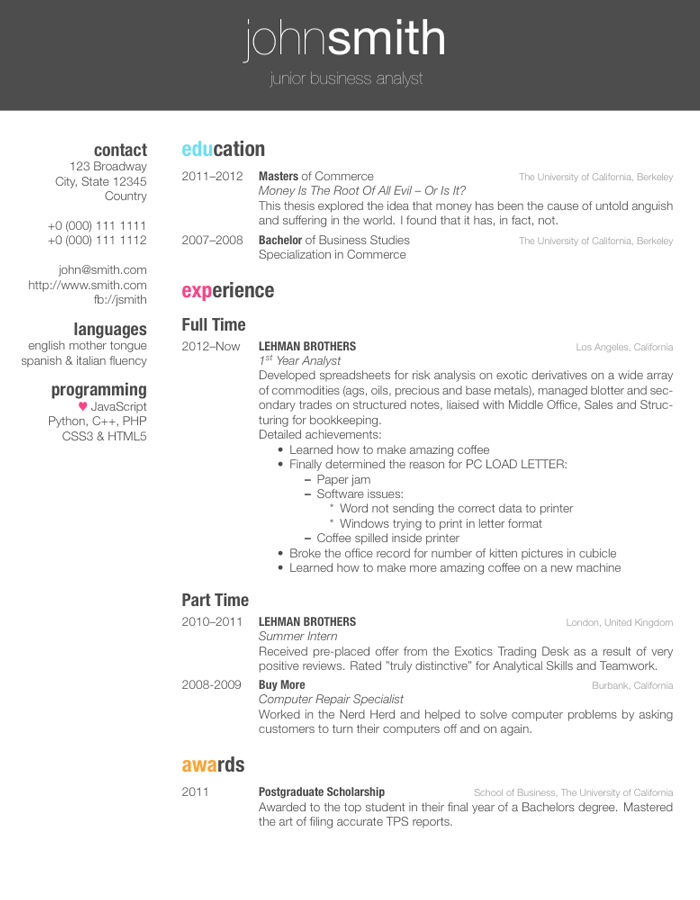
\includegraphics[height=2in]{cv_101}
        \caption{Beautiful!}
        \label{fig:left}
    \end{subfigure}
    ~
    \begin{subfigure}{0.45\textwidth}
        \centering
        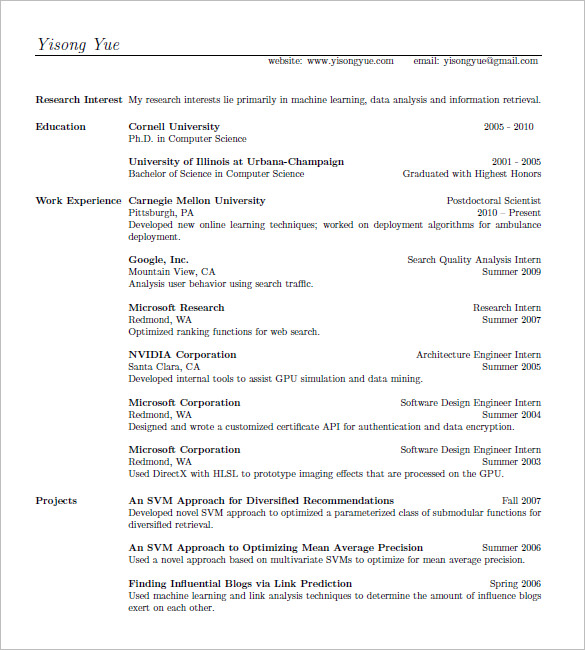
\includegraphics[height=2in]{cv_102}
        \caption{Amazing!}
        \label{fig:right}
    \end{subfigure}
    \caption{Each Better Than the Other!}
    \label{fig:combined}
\end{figure}

% -----------------------------% 
\subsection{Jupyter notebooks}
    \#ToDo

% -----------------------------%
\begin{thebibliography}{20}

\bibitem{referencing}
All About Referencing\\
\url{https://www.sharelatex.com/learn/Cross\_referencing\_sections\_and\_equations}

\bibitem{commands}
{\LaTeX} Commands, Macros, and Parameters\\
\url{https://www.sharelatex.com/learn/Commands}

\bibitem{tablegenerator}
Table Generator\\
\url{http://www.tablesgenerator.com/}

\bibitem{sourcecode}
Including Source Code:\\
\url{https://www.sharelatex.com/learn/Code\_listing}

\bibitem{syntax}
Source code with syntax highlighting:\\ \url{https://www.sharelatex.com/learn/Code\_Highlighting\_with\_minted}

\bibitem{learnalgorithmx}
Using the \verb$algorithmx$ package:
\url{https://en.wikibooks.org/wiki/LaTeX/Algorithms#Typesetting_using_the_algorithmicx_package}

\bibitem{tables}
Working with Tables\\ \url{https://en.wikibooks.org/wiki/LaTeX/Tables}

\bibitem{amspackages}
{\TeX} StackExchange: 'What does every AMS package do?'\\ \url{https://tex.stackexchange.com/questions/32100/what-does-each-ams-package-do}

\bibitem{theoremenvs}
Tweaking Theorem Environments\\ \url{https://en.wikibooks.org/wiki/LaTeX/Theorems}

\bibitem{posters}
Learn How to Make Posters\\
\url{la}

\bibitem{posterexample}
Example Project: Poster\\
\url{https://www.sharelatex.com/project/59096b20e750871a7e4b8a27}

\bibitem{joyoftex}
Spivak, Michael D. The joy of {\TeX}: a gourmet guide to typesetting with the AMS-TEX macro package. Providence, RI: American mathematical society, 1996. Print.

\end{thebibliography}

\end{document}
